\chapter{Methodology and Implementation}
\label{chap:methodology}

\section{System Overview}
\paragraph{} The proposed system is implemented as a full-stack document intelligence application. The frontend provides user-facing workflows for upload, dashboard monitoring, document review, search, and Agentic RAG. The backend exposes REST APIs and executes the document processing pipeline. The database stores uploaded document metadata, extracted fields, processing logs, chat history, and processing status.

\begin{figure}[h]
\centering
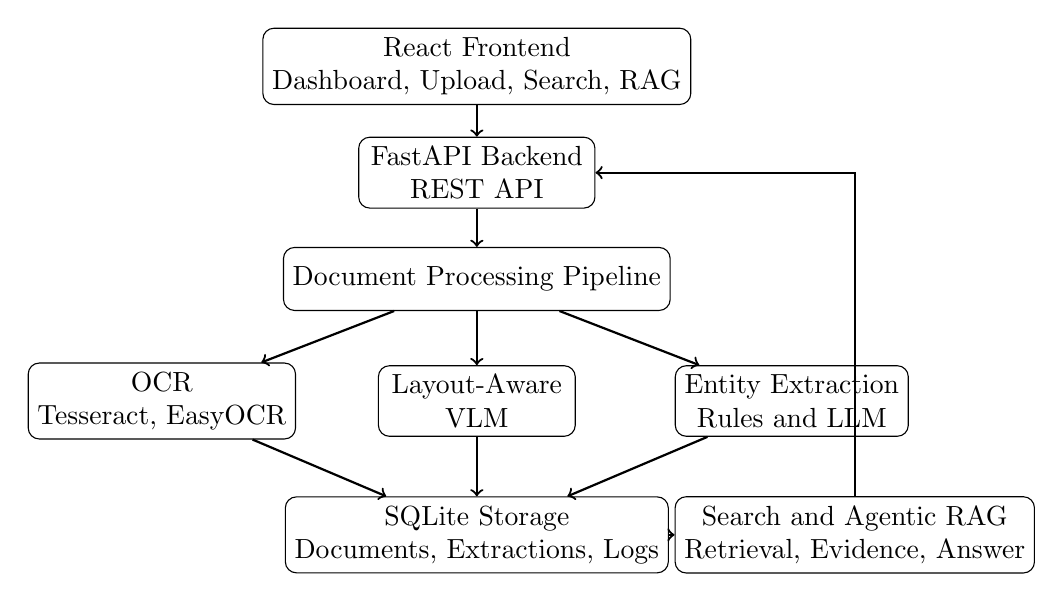
\begin{tikzpicture}[
    block/.style={rectangle, draw, rounded corners, align=center, minimum width=3.0cm, minimum height=0.8cm},
    smallblock/.style={rectangle, draw, rounded corners, align=center, minimum width=2.5cm, minimum height=0.75cm},
    arrow/.style={->, thick}
]
\node[block] (ui) at (0,0) {React Frontend\\Dashboard, Upload, Search, RAG};
\node[block] (api) at (0,-1.35) {FastAPI Backend\\REST API};
\node[block] (pipeline) at (0,-2.7) {Document Processing Pipeline};
\node[smallblock] (ocr) at (-4.0,-4.25) {OCR\\Tesseract, EasyOCR};
\node[smallblock] (vlm) at (0,-4.25) {Layout-Aware\\VLM};
\node[smallblock] (extract) at (4.0,-4.25) {Entity Extraction\\Rules and LLM};
\node[block] (db) at (0,-5.95) {SQLite Storage\\Documents, Extractions, Logs};
\node[block] (rag) at (4.8,-5.95) {Search and Agentic RAG\\Retrieval, Evidence, Answer};

\draw[arrow] (ui) -- (api);
\draw[arrow] (api) -- (pipeline);
\draw[arrow] (pipeline) -- (ocr);
\draw[arrow] (pipeline) -- (vlm);
\draw[arrow] (pipeline) -- (extract);
\draw[arrow] (ocr) -- (db);
\draw[arrow] (vlm) -- (db);
\draw[arrow] (extract) -- (db);
\draw[arrow] (db) -- (rag);
\draw[arrow] (rag) |- (api);
\end{tikzpicture}
\caption{High-level architecture of the document intelligence system}
\label{fig:architecture}
\end{figure}

\section{Technology Stack}
\paragraph{} The frontend is built using React and Vite. The backend is implemented in Python using FastAPI. SQLAlchemy provides database access, and SQLite is used for local persistence. OCR is performed with Tesseract and EasyOCR. Layout-aware classification and feature extraction use LayoutLMv3. Semantic retrieval uses sentence embeddings, and the local language model backend is used for grounded answer generation.

\begin{table}[h]
\centering
\begin{tabular}{ll}
\toprule
\textbf{Layer} & \textbf{Technology Used} \\
\midrule
Frontend & React, Vite, React Router \\
Backend API & FastAPI, Pydantic models \\
Database & SQLite, SQLAlchemy ORM \\
Text extraction & PyPDF2 for digital PDFs, OCR for scanned documents \\
OCR & Tesseract, EasyOCR \\
Document AI & LayoutLMv3 \\
Retrieval & Keyword search, database fallback, semantic chunk retrieval \\
Question answering & Local LLM-backed RAG and Agentic RAG \\
\bottomrule
\end{tabular}
\caption{Technology stack used in the prototype}
\label{tab:technology_stack}
\end{table}

\section{Functional Modules}
\paragraph{} The application is organised into the following functional modules:

\begin{enumerate}
    \item \textbf{Document upload}: accepts supported document formats and stores the original file with a unique identifier.
    \item \textbf{Processing pipeline}: performs text detection, extraction, table extraction, text merge, entity extraction, boundary detection, validation, indexing, and status update.
    \item \textbf{Document management}: lists uploaded documents, shows document details, extracted fields, and processing logs, and supports deletion or reprocessing.
    \item \textbf{Validation}: applies field-specific validation rules and flags low-confidence or invalid values.
    \item \textbf{Search}: retrieves documents using keyword and database-backed search.
    \item \textbf{Question answering}: answers questions for a single document or across all documents using RAG.
    \item \textbf{Agentic RAG}: performs query planning, structured lookup, evidence retrieval, evidence grading, and grounded answering.
    \item \textbf{Evaluation}: exposes metrics for extraction, search, throughput, and review rate.
\end{enumerate}

\section{Database Design}
\paragraph{} The system uses four main database entities. The \texttt{Document} table stores file metadata, document type, processing status, page count, processing time, upload time, processed time, and full extracted text. The \texttt{Extraction} table stores field name, field value, confidence, source, page number, bounding box, and review flag. The \texttt{ProcessingLog} table records pipeline steps and messages for auditability. The \texttt{ChatHistory} table stores question-answer interactions.

\paragraph{} The document status is represented using values such as uploaded, processing, completed, failed, and review needed. The document type is represented using values such as invoice, contract, form, report, and other. These enums make the UI and API responses easier to interpret.

\section{Document Processing Pipeline}
\paragraph{} The backend pipeline starts when a user uploads a file. A unique document identifier is created, the file is stored, a database record is inserted, and a background task is scheduled for processing. The major steps are shown in \cref{alg:document_pipeline}.

\begin{algorithm}[h]
\caption{Document Processing Pipeline}
\label{alg:document_pipeline}
\begin{algorithmic}[1]
\State Receive uploaded document and create database record
\State Mark document status as processing
\State Detect whether the PDF contains embedded text
\If{embedded text is available}
    \State Extract text directly from PDF pages
    \State Classify the first page using the layout-aware model
\Else
    \State Convert pages to images
    \State Run OCR and layout-aware processing on each page
    \State Fuse OCR and layout results
\EndIf
\State Extract table text where available
\State Merge page text and table text into full document text
\State Extract structured entities using rules and optional LLM extraction
\State Detect possible multi-document boundaries
\State Save extracted fields with confidence values
\State Validate fields using business rules
\State Index the document for keyword and semantic search
\State Mark the document as completed or review needed
\end{algorithmic}
\end{algorithm}

\section{Digital PDF and Scanned Document Handling}
\paragraph{} The pipeline uses two processing paths. For digital PDFs, embedded text is extracted directly. This is faster and avoids unnecessary OCR when reliable text is already present. For scanned documents, pages are converted to images and passed through OCR and layout-aware analysis. This design improves efficiency because digital PDFs and scanned files have different processing needs.

\paragraph{} For scanned pages, Tesseract extracts text, word confidence, and bounding boxes. EasyOCR is used as an alternate recogniser. The OCR service compares the resulting text and selects the more informative output as the primary OCR result. The layout-aware service classifies document type and captures layout features. The fusion service combines OCR text with layout metadata and flags low-confidence words.

\section{Entity Extraction}
\paragraph{} Entity extraction is performed over the merged document text. Rule-based extraction identifies common business fields such as dates, amounts, email addresses, vendor names, buyer names, parties, purchase order numbers, and invoice numbers. Extracted entities are normalised before storage. An optional LLM extraction step can contribute additional candidate fields not found by the rule-based extractor.

\paragraph{} Each extracted field is stored with a confidence value and a source label. If the confidence value is below the configured threshold \(\theta\), the field is marked as requiring review. This allows the system to support human-in-the-loop verification instead of silently accepting uncertain outputs.

\section{Validation Rules}
\paragraph{} Validation rules are applied after extraction. Date fields are checked for parseability and future dates. Amounts are checked for numeric format, non-negativity, and unusually high values. Email addresses are checked using a regular expression. Vendor and buyer names are checked against simple organisation-name heuristics and mock reference data. Purchase order numbers are checked against a mock list. Contract parties are checked for the presence of two plausible organisation names.

\paragraph{} The validation stage does not discard uncertain fields. Instead, it updates the corresponding extraction record to indicate that review is needed. This design preserves extracted evidence while clearly informing the user that the value should be verified manually.

\section{Search and Indexing}
\paragraph{} After extraction and validation, the document is indexed for search. The keyword search layer indexes full text and extracted fields. If in-memory keyword search does not return results, the database-backed search function is used as a fallback. For RAG, document text is split into chunks and indexed with embeddings. These chunks are later retrieved as evidence for question answering.

\section{Agentic RAG Workflow}
\paragraph{} The Agentic RAG workflow improves over direct question answering by adding intermediate reasoning steps. First, the question is normalised and planned. The planner identifies intents such as field lookup, comparison, risk review, summary, or grounded QA. If the question is a structured field lookup and the extracted field exists, the answer is produced directly from the \texttt{Extraction} table. This is faster and more reliable for exact fields.

\paragraph{} If structured lookup is not sufficient, the system retrieves candidate chunks using semantic retrieval. Candidate evidence is graded using a score that combines vector similarity, question-term coverage, and intent-specific bonuses. Only the top graded evidence is used to build the context for the answer generator. The final response contains the answer, intent, confidence, evidence snippets, trace steps, latency, and error status if applicable.

\begin{algorithm}[h]
\caption{Agentic RAG Question Answering}
\label{alg:agentic_rag}
\begin{algorithmic}[1]
\State Receive user question and optional document filter
\State Detect query intent and field target
\If{intent is field lookup and structured extraction exists}
    \State Return answer from extracted fields with confidence and evidence
\Else
    \State Retrieve candidate chunks using semantic search
    \State Grade evidence using similarity, coverage, and intent bonuses
    \If{best evidence score is below threshold}
        \State Return insufficient-evidence response
    \Else
        \State Build grounded context from selected evidence
        \State Generate answer using only selected evidence
        \State Return answer, confidence, evidence, and trace steps
    \EndIf
\EndIf
\end{algorithmic}
\end{algorithm}

\section{API Design}
\paragraph{} The backend exposes REST APIs under the prefix \texttt{/api/v1}. The major endpoints include document upload, document listing, document detail, deletion, reprocessing, validation, document-specific question answering, all-document question answering, agent-based answering, Agentic RAG answering, search, statistics, and evaluation metrics. These endpoints allow the frontend and external clients to use the same processing backend.

\section{User Interface}
\paragraph{} The frontend contains pages for Dashboard, Upload, Documents, Document Detail, Search, and Agentic RAG. The dashboard displays processing statistics. The upload page lets users submit documents. The document pages allow review of extracted values and processing logs. The search page supports document retrieval. The Agentic RAG page allows users to ask questions and inspect evidence-backed answers.

\section{Deployment Model}
\paragraph{} The application can run locally as a development prototype. The production-style path serves the built React frontend from the FastAPI backend, making the backend a single service for both APIs and the single-page application. This design simplifies local demonstration and can also be adapted for cloud deployment using a container image.
